% GNUPLOT: LaTeX picture with Postscript
\begingroup
  \makeatletter
  \providecommand\color[2][]{%
    \GenericError{(gnuplot) \space\space\space\@spaces}{%
      Package color not loaded in conjunction with
      terminal option `colourtext'%
    }{See the gnuplot documentation for explanation.%
    }{Either use 'blacktext' in gnuplot or load the package
      color.sty in LaTeX.}%
    \renewcommand\color[2][]{}%
  }%
  \providecommand\includegraphics[2][]{%
    \GenericError{(gnuplot) \space\space\space\@spaces}{%
      Package graphicx or graphics not loaded%
    }{See the gnuplot documentation for explanation.%
    }{The gnuplot epslatex terminal needs graphicx.sty or graphics.sty.}%
    \renewcommand\includegraphics[2][]{}%
  }%
  \providecommand\rotatebox[2]{#2}%
  \@ifundefined{ifGPcolor}{%
    \newif\ifGPcolor
    \GPcolortrue
  }{}%
  \@ifundefined{ifGPblacktext}{%
    \newif\ifGPblacktext
    \GPblacktexttrue
  }{}%
  % define a \g@addto@macro without @ in the name:
  \let\gplgaddtomacro\g@addto@macro
  % define empty templates for all commands taking text:
  \gdef\gplbacktext{}%
  \gdef\gplfronttext{}%
  \makeatother
  \ifGPblacktext
    % no textcolor at all
    \def\colorrgb#1{}%
    \def\colorgray#1{}%
  \else
    % gray or color?
    \ifGPcolor
      \def\colorrgb#1{\color[rgb]{#1}}%
      \def\colorgray#1{\color[gray]{#1}}%
      \expandafter\def\csname LTw\endcsname{\color{white}}%
      \expandafter\def\csname LTb\endcsname{\color{black}}%
      \expandafter\def\csname LTa\endcsname{\color{black}}%
      \expandafter\def\csname LT0\endcsname{\color[rgb]{1,0,0}}%
      \expandafter\def\csname LT1\endcsname{\color[rgb]{0,1,0}}%
      \expandafter\def\csname LT2\endcsname{\color[rgb]{0,0,1}}%
      \expandafter\def\csname LT3\endcsname{\color[rgb]{1,0,1}}%
      \expandafter\def\csname LT4\endcsname{\color[rgb]{0,1,1}}%
      \expandafter\def\csname LT5\endcsname{\color[rgb]{1,1,0}}%
      \expandafter\def\csname LT6\endcsname{\color[rgb]{0,0,0}}%
      \expandafter\def\csname LT7\endcsname{\color[rgb]{1,0.3,0}}%
      \expandafter\def\csname LT8\endcsname{\color[rgb]{0.5,0.5,0.5}}%
    \else
      % gray
      \def\colorrgb#1{\color{black}}%
      \def\colorgray#1{\color[gray]{#1}}%
      \expandafter\def\csname LTw\endcsname{\color{white}}%
      \expandafter\def\csname LTb\endcsname{\color{black}}%
      \expandafter\def\csname LTa\endcsname{\color{black}}%
      \expandafter\def\csname LT0\endcsname{\color{black}}%
      \expandafter\def\csname LT1\endcsname{\color{black}}%
      \expandafter\def\csname LT2\endcsname{\color{black}}%
      \expandafter\def\csname LT3\endcsname{\color{black}}%
      \expandafter\def\csname LT4\endcsname{\color{black}}%
      \expandafter\def\csname LT5\endcsname{\color{black}}%
      \expandafter\def\csname LT6\endcsname{\color{black}}%
      \expandafter\def\csname LT7\endcsname{\color{black}}%
      \expandafter\def\csname LT8\endcsname{\color{black}}%
    \fi
  \fi
    \setlength{\unitlength}{0.0500bp}%
    \ifx\gptboxheight\undefined%
      \newlength{\gptboxheight}%
      \newlength{\gptboxwidth}%
      \newsavebox{\gptboxtext}%
    \fi%
    \setlength{\fboxrule}{0.5pt}%
    \setlength{\fboxsep}{1pt}%
\begin{picture}(8640.00,5760.00)%
    \gplgaddtomacro\gplbacktext{%
      \csname LTb\endcsname%%
      \put(762,576){\makebox(0,0)[r]{\strut{}0.00}}%
      \csname LTb\endcsname%%
      \put(762,1056){\makebox(0,0)[r]{\strut{}3.00}}%
      \csname LTb\endcsname%%
      \put(762,1536){\makebox(0,0)[r]{\strut{}6.00}}%
      \csname LTb\endcsname%%
      \put(1508,390){\makebox(0,0){\strut{}0.002}}%
      \csname LTb\endcsname%%
      \put(3117,390){\makebox(0,0){\strut{}0.0025}}%
      \csname LTb\endcsname%%
      \put(4726,390){\makebox(0,0){\strut{}0.003}}%
      \csname LTb\endcsname%%
      \put(6335,390){\makebox(0,0){\strut{}0.0035}}%
      \csname LTb\endcsname%%
      \put(7944,390){\makebox(0,0){\strut{}0.004}}%
    }%
    \gplgaddtomacro\gplfronttext{%
      \csname LTb\endcsname%%
      \put(168,1296){\rotatebox{-270}{\makebox(0,0){\strut{}Error (\%)}}}%
      \csname LTb\endcsname%%
      \put(4726,111){\makebox(0,0){\strut{}Absorbance / 1 cm}}%
    }%
    \gplgaddtomacro\gplbacktext{%
      \csname LTb\endcsname%%
      \put(762,2016){\makebox(0,0)[r]{\strut{}0.05}}%
      \csname LTb\endcsname%%
      \put(762,2929){\makebox(0,0)[r]{\strut{}0.10}}%
      \csname LTb\endcsname%%
      \put(762,3841){\makebox(0,0)[r]{\strut{}0.15}}%
      \csname LTb\endcsname%%
      \put(762,4754){\makebox(0,0)[r]{\strut{}0.20}}%
      \csname LTb\endcsname%%
      \put(762,5666){\makebox(0,0)[r]{\strut{}0.25}}%
      \csname LTb\endcsname%%
      \put(1508,1830){\makebox(0,0){\strut{}}}%
      \csname LTb\endcsname%%
      \put(3117,1830){\makebox(0,0){\strut{}}}%
      \csname LTb\endcsname%%
      \put(4726,1830){\makebox(0,0){\strut{}}}%
      \csname LTb\endcsname%%
      \put(6335,1830){\makebox(0,0){\strut{}}}%
      \csname LTb\endcsname%%
      \put(7944,1830){\makebox(0,0){\strut{}}}%
      \csname LTb\endcsname%%
      \put(1250,4936){\makebox(0,0)[l]{\strut{}$a = 0.00013 \pm 0.00007$}}%
      \csname LTb\endcsname%%
      \put(1250,4571){\makebox(0,0)[l]{\strut{}$b = 0.0189 \pm 0.0005$}}%
      \csname LTb\endcsname%%
      \put(1250,4206){\makebox(0,0)[l]{\strut{}$\chi^2$ / DOF = 390.17288 / 9}}%
    }%
    \gplgaddtomacro\gplfronttext{%
      \csname LTb\endcsname%%
      \put(168,3841){\rotatebox{-270}{\makebox(0,0){\strut{}Concentration (\%)}}}%
      \csname LTb\endcsname%%
      \put(1658,5301){\makebox(0,0)[r]{\strut{}Data}}%
    }%
    \gplbacktext
    \put(0,0){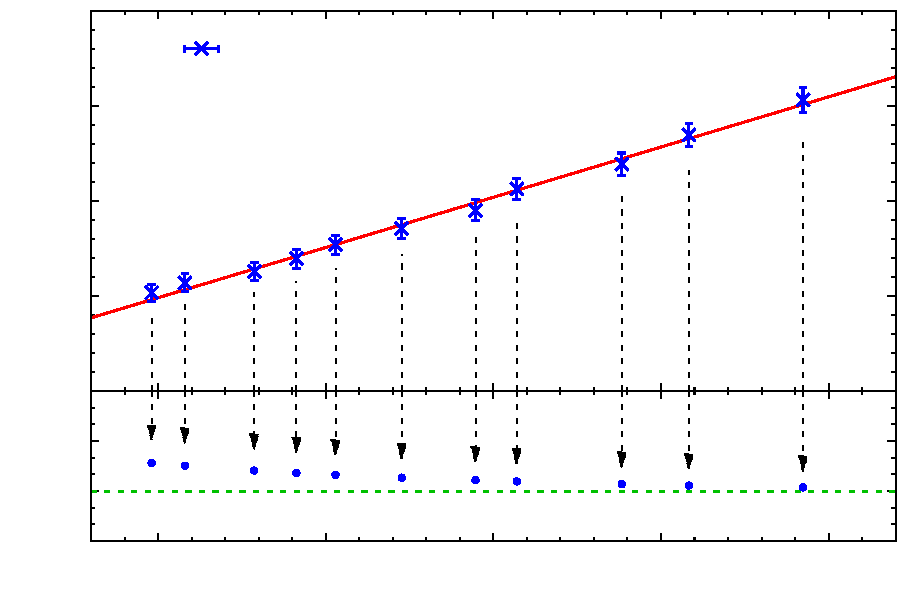
\includegraphics{pics/gad_10cm}}%
    \gplfronttext
  \end{picture}%
\endgroup
